%
% LaTeX report template 
%

% This is a comment: in LaTeX everything that in a line comes
% after a "%" symbol is treated as comment

\documentclass[11pt, a4paper]{article}
\usepackage{graphicx}
\usepackage{amsmath}
\usepackage{listings}
\usepackage{url}

\title{EE2703 Final Exam} % Title

\author{EE19B049(Jahnavi Pragada)} % Author name

\date{\today} % Date for the report
\begin{document}	
		
\maketitle % Insert the title, author and date
\section*{Abstract}
%Create new section;it is autonumbered
This problem is about radiation from a loop antenna of length \lambda.\\

The main content of the assignment is: 
\begin{itemize}
\item Finding the current in loop using vectors.
\item Finding magnetic field due to the loop along z-axis.
\item Fitting the field to a fit of the type $B_z$ \approx  $cz^b$. 
\end{itemize}

\section*{Given data for solving the problem}
A long wire carries a current\\

$I =\frac{4\pi}{\mu_0}cos(\phi)exp(jωt)$ 
\\ 

through a loop of wire. Here, $\phi$ is the angle in polar coordinates i.e., in ( $r$ , $\phi$ , $z$) coordinates.
The wire is on the $x-y$ plane and centered at the origin. The radius of the loop is 10 cm
and is also equal to $1/k = c/\omega$. (This means that the circumference is $\lambda$)\\

The problem is to compute and plot the magnetic field $\vec{B}$ along the $z$ axis from 1cm to 1000 cm, plot it and then fit the data to $|\vec{B}| = cz^b$.
of grid will give.\\

The computation involves the calculation of the vector potential\\

$\vec{A}(r, \phi, z) = \frac{\mu_0}{4\pi}\int \frac{(I\phi) \phi exp(−jkR) a d\phi}{R} $)\\

where $\vec{R} =|\vec{r}-\vec{r_0}|$and $k = \omega /c = 0.1$. $\vec{r}$  is the point where we want the field, and $\vec{r'} = a\vec{r'}$ is the point on the loop. Due to the This can be reduced to a sum:\\

$\vec{A}_{ijk} = \sum\limits^{N-1}_{l=0} \frac{cos(\phi'_l)exp(-jkR_{ijkl})\vec{dl'}}{R_{ijkl}}$.....(1)
\\

where $\vec{r}$ is at $r_i,\phi_j,z_k$ and $\vec{r'}$ is at $acos\phi'_l x̂ + asin\phi'_l ŷ$. Note that Eq. (1) is valid for any $(x_i,y_j,z_k)$ ,and is summed over the current elements in the loop. You must implement this as a vector operation over both $l$ and over a vector of $(x_i,y_j,z_k)$ values.
From $\vec{A}$, you can obtain $\vec{B}$ as\\

 $\vec{B} = \nabla X \vec{A}$
\\

Along the z axis this becomes ( $\vec{A}$ is along $φ̂ $and the curl gives only $aB_z$ component along $ẑ$.\\

$B_z(z) =\frac{A_y(\triangle x,0,z) - A_x (0,\triangle y,z) - A_y(-\triangle x,0,z) + A_x(0, −\triangle y, z)}{4\triangle x\triangle y}$.....(2)


\section*{Part 2}
\begin{itemize}
\item Breaking the volume into a 3 by 3 by 1000 mesh, with mesh points separated by 1cm.(The 3 by 3 grid in x − y is can be used to compute the curl using Eq.2).
\end{itemize}
The following code snippet do the process:
\begin{verbatim}	
x=np.linspace(-1,1,num=3)
y=np.linspace(-1,1,num=3)
z=np.linspace(0,5000,num=1000)
X,Y,Z=np.meshgrid(x,y,z)
\end{verbatim}
   
   
\section*{Part 3 and 4}
\begin{itemize}
\item Obtained vectors $\vec{r_l}$ and $\vec{d_l}$ which will be used in further calculations.
\item We found the Current in the loop with the equation given in the data and ploted it.
\end{itemize}

The python code snippet for finding vectors $\vec{r_l}$ and $\vec{d_l}$ is as follows:
\begin{verbatim}	
r_l = rad*np.array([np.cos(phi), np.sin(phi), np.zeros(len(phi))]).T
d_l = 2*pi*rad*(1/secs)*np.array([-np.sin(phi), np.cos(phi), np.zeros(len(phi))]).T
\end{verbatim}

The python code snippet for finding and ploting current is as follows:
\begin{verbatim}	
I = 4*pi*(1/(4*pi*1e-7))*np.array([-np.cos(phi)*np.sin(phi), np.cos(phi)*np.cos(phi)]).T
plt.figure(0)
plt.quiver(r_l[:,0],r_l[:,1],I[:,0],I[:,1])
plt.xlabel("x $\longrightarrow$")
plt.ylabel("y $\longrightarrow$")
plt.title("Quiver Plot of Current in the Loop")
plt.grid()
plt.show()
\end{verbatim}

The quiver plot of current in the loop obtained is as follows:   
	\begin{figure}[!tbh]
   	\centering
   	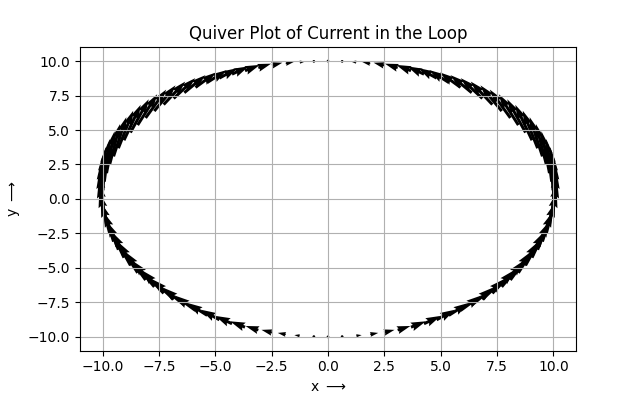
\includegraphics[scale=0.9]{Figure_0.png}   
   	\caption{Current plot}
   	\label{fig:sample}
   \end{figure} 
  
\section*{Part 5 and 6}
\begin{itemize}
\item Calculated magnitude of $\vec{R}$ which will be used to find magnetic potential.
\item Clculated magnetic potential at a point in loop which will further be added to get Magnetic potential.
\end{itemize}
The python code snippet of function that can find these is as shown below:
\begin{verbatim}	
def calc(l):
    k = 1/rad
    x_l, y_l, z_l = r_l[l]
    R_ijkl = np.sqrt((X-x_l)**2 + (Y - y_l)**2 + (Z - z_l)**2)
    A_ijkl = np.cos(l*2*pi/100)*np.exp(-1j*k*R_ijkl)/R_ijkl
    return A_ijkl	
\end{verbatim} 


\section*{Part 7}
\begin{itemize}
\item Adding up the potential at any point($\vec{A_{ijkl}}$) obtained from above function to obtain the potential($\vec{A_{ijk}}$)
\end{itemize}
The python code snippet is as follows:
\begin{verbatim}	
A_x = np.zeros(X.shape)
A_y = np.zeros(Y.shape)
A_z = np.zeros(Z.shape)
for n in range(secs): 
  A_ijkl = calc(n)
  A_x = A_x + A_ijkl*d_l[n,0]
  A_y = A_y + A_ijkl*d_l[n,1]
  A_z = A_z + A_ijkl*d_l[n,2]
\end{verbatim}

\section*{Part 8 and 9} 
\begin{itemize}
\item Computing Magnetic Field $\vec{B}$ along z-axis.
\item Plotting a loglog plot of $\vec{B_z}$ and z.
\end{itemize}
The python code snippet is as follows:
\begin{verbatim}	

Bz = 0.25*(A_y[1,0,:]-A_x[0,1,:]-A_y[-1,0,:]+A_x[0,-1,:])

plt.figure(1)
plt.loglog(z, np.abs(Bz))
plt.xlabel("z $\longrightarrow$")
plt.ylabel("Bz $\longrightarrow$")
plt.title("loglog plot of Magnetic field")
plt.grid()
plt.show()
\end{verbatim}

The loglogplot of Magnetic field alongz-axis is as follows :
	\begin{figure}[!tbh]
   	\centering
   	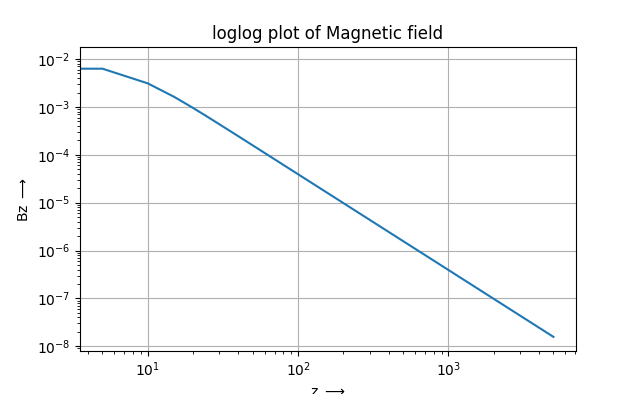
\includegraphics[scale=0.9]{Figure_1.png}   
   	\caption{Magnetic field plot}
   	\label{fig:sample}
   \end{figure} 
   
\section*{Part 10}
\begin{itemize}
\item Fitting the field obtained to a type given i.e.,$B_z$ \approx  $cz^b$
\end{itemize}
The following code snippet do the process:
\begin{verbatim}	
B = np.hstack([np.ones(len(Bz[999:]))[:,np.newaxis],np.log(z[999:])[:,np.newaxis]])
log_c , b = np.linalg.lstsq(B,np.log(np.abs(Bz[999:]))) [0]
c=np.exp(log_c)
\end{verbatim}
 
\end{document}
